\documentclass[a4paper, 12pt]{book}
\usepackage[T1]{fontenc}
\usepackage{titlesec}
\usepackage{ragged2e}
\usepackage{blindtext}
\usepackage{graphicx}
\usepackage{wrapfig}
\usepackage[rightcaption]{sidecap}


\titleformat
{\chapter} % command is the sectioning command to be redefined
[display] % shape is sectioning the paragraph shape
{\bfseries\Large\itshape} % format to be applied to title, label and text
{Name: \ } % label - specify sectioning label
{0.5ex} % sep - horizontal separation between label and title body and it must be a length and not be empty
{
    \rule{\textwidth}{1pt}
    \vspace{1ex}
    \centering
} % before-code uses {} and code precedes the title body
[
    \vspace{-0.5ex}%
    \rule{\textwidth}{0.3pt}
] % after-code uses [] and follows the title body

\titleformat{\section}
{\normalfont\bfseries}
{\thesection.}{0.5em}{}

\titlespacing{\section}
% structure is \titlespacing{command}{left}{before-sep}{after-sep}

\begin{document}
    \chapter{Read and Write}
    \section{Complete each sentence with a word from the list.}
    
    \begin{center}
        \textbf{\Huge{cat \hspace{0.8cm} bat \hspace{0.8cm} map}}
    \end{center}
    \vspace{8mm} %5mm vertical space
    \begin{flushleft}
        \textbf{\Huge {I am a .................... . }}
\includegraphics[width=0.15\textwidth]{cat.png}
    \end{flushleft}
    \begin{flushleft}
        \textbf{\Huge {I am a .................... . }}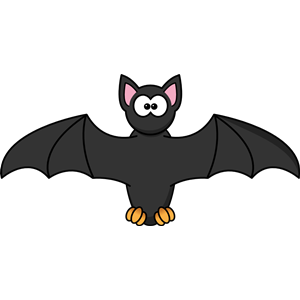
\includegraphics[width=0.15\textwidth]{bat.png}
    \end{flushleft}
    \begin{flushleft}
        \textbf{\Huge {I am a .................... . }}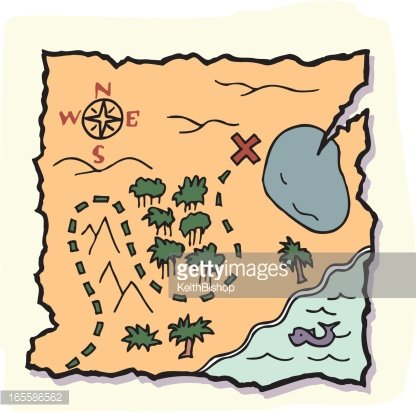
\includegraphics[width=0.15\textwidth]{map.jpeg}
    \end{flushleft}
    \begin{flushleft}
        \vspace{4mm}
        \textbf{\Huge {I am a fat .................... . }}
\includegraphics[width=0.15\textwidth]{fat-cat.jpeg}
    \end{flushleft}
    \section{Complete each sentence with one of the words.}
    
    \begin{center}
        \textbf{\Huge{I \hspace{0.8cm} am \hspace{0.8cm} a}}
    \end{center}
    \vspace{6mm} %5mm vertical space
    \begin{flushleft}
        \textbf{\Huge {I am .................... cat. }}
        \vspace{10mm}
    \begin{flushleft}
        \textbf{\Huge {I .................... a bat. }}
        \vspace{10mm}
    \begin{flushleft}
        \textbf{\Huge {.................... am a fat cat. }}
        \vspace{10mm}
    \begin{flushleft}
        \textbf{\Huge {I .................... Sam. }}
    \end{flushleft}

    \vspace{5mm} %5mm vertical space
    \section{Finish the \textbf{ap words}. }
    
   
    
    \begin{flushleft}
        
\includegraphics[width=0.15\textwidth]{nap.jpeg}
        \hspace{0.8cm}
        \textbf{\Huge {.................... ap}}
    \end{flushleft}
    \begin{flushleft}
        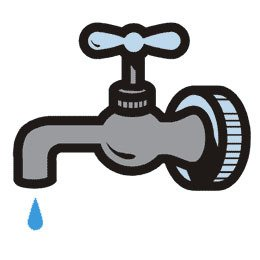
\includegraphics[width=0.15\textwidth]{tap.jpeg}
        \hspace{0.8cm}
        \textbf{\Huge {.................... ap}}
    \end{flushleft}
    \begin{flushleft}
        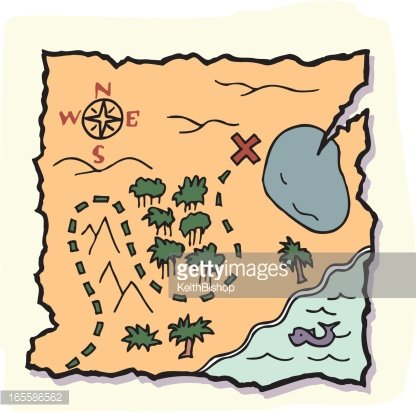
\includegraphics[width=0.15\textwidth]{map.jpeg}
        \hspace{0.8cm}
        \textbf{\Huge {.................... ap}}
    \end{flushleft}
    \vspace{3mm}
    \begin{flushleft}
        
\includegraphics[width=0.15\textwidth]{cap.png}
        \hspace{0.8cm}
        \textbf{\Huge {.................... ap}}
    \end{flushleft}

\end{document}